\section{Methods}
\label{sec:methods}
In this section, accurate methods used to compute the magnetic vector potential and the magnetic field
of a straight wire segment and a circular wire loop are presented.
Furthermore, methods to evaluate the magnetostatic quantities in Cartesian coordinates are provided.
The section is concluded by a description of the verification procedure
employed to benchmark these methods.

\subsection{Straight Wire Segment}
The straight wire segment is handled first.
The basic geometry of a single wire segment is shown in Fig.~\ref{fig:straightWireSegment}.
\begin{figure}[htbp]
 \centering
 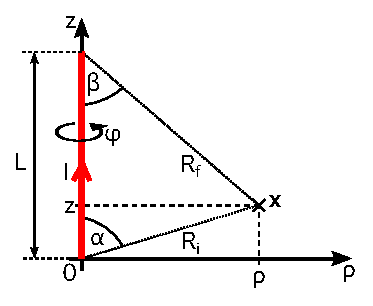
\includegraphics{img/straightWireSegment.eps}
 \caption{Geometry of a single wire segment. After Fig.~1 in Ref.~\cite{hanson_hirshman_2002}.}
 \label{fig:straightWireSegment}
\end{figure}

\subsubsection{Magnetic Vector Potential}
The magnetic vector potential of a straight wire segment
only has component~$A_z$ parallel to the wire:
\begin{equation}
 \mathbf{A} = A_z \hat{\mathbf{e}}_z \, .
\end{equation}
It is given by:
\begin{equation}
  A_z(\rho, z) = \frac{\mu_0 I}{4 \pi} \ln \left( \frac{1 + \epsilon}{1 - \epsilon} \right)
\end{equation}
with
\begin{align}
  \epsilon =&\, \frac{L}{R_\mathrm{i} + R_\mathrm{f}} \\
       R_\mathrm{i} =&\, \sqrt{\rho^2 + z^2} \\
       R_\mathrm{f} =&\, \sqrt{\rho^2 + (1 - z)^2} \, .
\end{align}
Here, we use normalized coordinates~$\rho' = \rho/L$ and~$z' = z/L$.
This leads to the following expressions
for~$r_\mathrm{i} = R_\mathrm{i}/L$ and~$r_\mathrm{f} = R_\mathrm{f}/L$:
\begin{align}
  r_\mathrm{i} =&\, \sqrt{{\rho'}^2 +      {z'}^2 }       \label{eqn:r_i_default} \\
  r_\mathrm{f} =&\, \sqrt{{\rho'}^2 + (1 - {z'})^2}       \label{eqn:r_f_default} \\
  \epsilon     =&\, \frac{1}{r_\mathrm{i} + r_\mathrm{f}} \label{eqn:eps_default}\, .
\end{align}
A common prefactor depending on the current~$I$ and~$\mu_0$ is split off:
\begin{equation}
  A_z(\rho, z) = \frac{\mu_0 I}{2 \pi} \tilde{A}_z (\rho', z')
\end{equation}
with
\begin{equation}
  \tilde{A}_z (\rho', z')
  = \frac{1}{2} \ln \left( \frac{1 + \epsilon}{1 - \epsilon} \right)
  = \textrm{atanh} (\epsilon) \, . \label{eqn:A_z_tilde}
\end{equation}
The rest of this section is dedicated to the accurate computation of $\tilde{A}_z (\rho', z')$.
One of several formulations is chosen depending on the evaluation location~$(\rho', z')$:
\begin{equation}
  \tilde{A}_z (\rho', z') =
  \begin{cases}
    \tilde{A}_\mathrm{z,ax}  (z')        &:\, \rho' = 0 , \textrm{ any } z'      \\
    \tilde{A}_\mathrm{z,rad} (\rho')     &:\, \textrm{any } \rho', z' \in \{0, 1\} \\
    \tilde{A}_\mathrm{z,f}   (\rho', z') &:\, \rho' \geq 1 \textrm{ or } z' \leq 1 \textrm{ or } z' > 2 \\
    \tilde{A}_\mathrm{z,n}   (\rho', z') &:\, \textrm{else} \, .
  \end{cases}
\end{equation}
For the case~$\rho'=0$, the following formulation is used:
\begin{equation}
  \tilde{A}_\mathrm{z,ax} (z') =
  \begin{cases}
    \tilde{A}_\mathrm{z,ax,f} (z') &:\, z' < -1 \textrm{ or } z' > 2 \\
    \tilde{A}_\mathrm{z,ax,n} (z') &:\, \textrm{else}
  \end{cases}
\end{equation}
with
\begin{equation}
  \tilde{A}_\mathrm{z,ax,f} (z') = \textrm{atanh}\left( \frac{1}{|z'| + |1 - z'|} \right)
\end{equation}
and
\begin{equation}
  \tilde{A}_\mathrm{z,ax,n} (z') = \frac{1}{2} \frac{z'}{|z'|} \ln \left(\left| \frac{z'}{1 - z'} \right| \right) \, .
\end{equation}
The following formulation is used for the cases $z'=0$ or $z'=1$:
\begin{equation}
  \tilde{A}_\mathrm{z,rad} (\rho') =
  \begin{cases}
    \tilde{A}_\mathrm{z,rad,f} (\rho')  &:\, \rho' > 1 \\
    \tilde{A}_\mathrm{z,rad,n} (\rho') &:\, \textrm{else}
  \end{cases}
\end{equation}
with
\begin{equation}
  \tilde{A}_\mathrm{z,rad,f} (z') = \textrm{atanh}\left( \frac{1}{\rho' + \sqrt{{\rho'}^2 + 1}} \right)
\end{equation}
and
\begin{equation}
  \tilde{A}_\mathrm{z,rad,n} (z') = \frac{1}{2} \ln \left(\frac{\rho' c + 1 + c}{\rho' c + 2 s^2 }\right) \, ,
\end{equation}
where
\begin{align}
  c =&\, \frac{1}{\sqrt{{\rho'}^2 + 1}} \\
  s =&\, \sin(\arctan(\rho')/2) \, .
\end{align}
The case of~$\tilde{A}_\mathrm{z,f}(\rho', z')$ is implemented as:
\begin{equation}
  \tilde{A}_\mathrm{z,f}(\rho', z') = \textrm{atanh} (\epsilon)
\end{equation}
with~$r_\mathrm{i}$, $r_\mathrm{f}$ and~$\epsilon$ from~\eqn{r_i_default}, \eqn{r_f_default} and~\eqn{eps_default}, respectively.
The final case is implemented as follows:
\begin{equation}
  \tilde{A}_\mathrm{z,n} (\rho', z') = \frac{1}{2} \left[ \ln\left(n + 2 \right) - \ln \left( n \right)  \right]
\end{equation}
with
\begin{align}
  n                       =&\, (r_\mathrm{i} - z') + (r_\mathrm{f} - (1 - z')) \\
  r_\mathrm{i} - z'       =&\, 2 r_\mathrm{i} \sin^2(\alpha/2) \label{eqn:ri_zp} \\
  r_\mathrm{f} - (1 - z') =&\, 2 r_\mathrm{f} \sin^2(\beta/2)  \label{eqn:rf_zp_1} \\
  \alpha =&\, \texttt{atan2}(\rho', z')   \label{eqn:sws_alpha} \\
  \beta  =&\, \texttt{atan2}(\rho', 1-z') \label{eqn:sws_beta} \, .
\end{align}

\subsubsection{Magnetic Field}
The magnetic field of a straight wire segment
is given by~\cite{hanson_hirshman_2002}:
\begin{equation}
 \mathbf{B}
 = \frac{\mu_0 I}{4 \pi}
   \hat{\mathbf{e}}_z \times \mathbf{R}_\mathrm{i}
   \frac{2 L (R_\mathrm{i} + R_\mathrm{f})}{R_\mathrm{i} R_\mathrm{f}} \frac{1}{\left(R_\mathrm{i} + R_\mathrm{f}\right)^2 - L^2} \, . \label{eqn:sws_B_phi}
\end{equation}
The vector~$\mathbf{R}_\mathrm{i}$ has components in directions parallel~($z$) and perpendicular~($\rho$) to the wire segment:
\begin{equation}
 \mathbf{R}_\mathrm{i}
 = z \,\hat{\mathbf{e}}_z + \rho \,\hat{\mathbf{e}}_\rho
\end{equation}
where $\rho$ and $z$ are cylindrical coordinates in the coordinate system aligned with the wire segment.
The vector-valued term in~\eqn{sws_B_phi} is reformulated as follows:
\begin{align}
 \hat{\mathbf{e}}_z \times \mathbf{R}_\mathrm{i}
 =&\, \hat{\mathbf{e}}_z \times \left( z \,\hat{\mathbf{e}}_z + \rho \,\hat{\mathbf{e}}_\rho \right) \nonumber \\
 =&\,      z \underbrace{\hat{\mathbf{e}}_z \times \hat{\mathbf{e}}_z}_{=0}
      + \rho \underbrace{\hat{\mathbf{e}}_z \times \hat{\mathbf{e}}_\rho}_{=\hat{\mathbf{e}}_\varphi}
 = \rho \,\hat{\mathbf{e}}_\varphi \, .
\end{align}
It follows that the magnetic field of a straight wire segment only has a component~$B_\varphi$ in tangential direction:
\begin{equation}
 \mathbf{B} = B_\varphi \hat{\mathbf{e}}_\varphi
\end{equation}
with
\begin{equation}
 B_\varphi (\rho, z)
 = \frac{\mu_0 I}{4 \pi}
   \frac{2 \rho L (R_\mathrm{i} + R_\mathrm{f})}{R_\mathrm{i} R_\mathrm{f}}
   \frac{1}{\left(R_\mathrm{i} + R_\mathrm{f}\right)^2 - L^2} \, .
\end{equation}
This is now reformulated to use normalized quantities
(as done above for the computation of the magnetic vector potential):
\begin{equation}
 B_\varphi
 = \frac{\mu_0 I}{4 \pi L}
   \left(\frac{1}{r_\mathrm{f}} + \frac{1}{r_\mathrm{i}} \right)
   \frac{2 \rho'}{\left( r_\mathrm{i} + r_\mathrm{f} \right)^2 - 1} \, .
\end{equation}
Again a normalization factor is split off:
\begin{equation}
  B_\varphi(\rho, z) = \frac{\mu_0 I}{4 \pi L} \tilde{B}_\varphi(\rho', z')
\end{equation}
with
\begin{equation}
  \tilde{B}_\varphi(\rho', z')
  = \left(\frac{1}{r_\mathrm{f}} + \frac{1}{r_\mathrm{i}} \right)
    \frac{2 \rho'}{\left( r_\mathrm{i} + r_\mathrm{f} \right)^2 - 1} \, .
\end{equation}
Consider the denominator in more detail:
\begin{align}
 \left(r_\mathrm{i} + r_\mathrm{f}\right)^2 - 1
 =&\, r_\mathrm{i}^2 + 2 r_\mathrm{i} r_\mathrm{f} + r_\mathrm{f}^2 - 1 \nonumber \\
 =&\, {\rho'}^2 + {z'}^2 + 2 r_\mathrm{i} r_\mathrm{f} + {\rho'}^2 + (1 - z')^2 - 1 \nonumber \\
 =&\, {\rho'}^2 + {z'}^2 + 2 r_\mathrm{i} r_\mathrm{f} + {\rho'}^2 \bcancel{+ 1} - 2 z' + {z'}^2 \bcancel{- 1} \nonumber \\
 =&\, 2 {\rho'}^2 + 2 {z'}^2 + 2 r_\mathrm{i} r_\mathrm{f} - 2 z' \nonumber \\
 =&\, 2 \left[ {\rho'}^2 + r_\mathrm{i} r_\mathrm{f} - z' (1 - z') \right] \, .
\end{align}
This leads to:
\begin{equation}
 \tilde{B}_\varphi(\rho', z')
  = \left(\frac{1}{r_\mathrm{f}} + \frac{1}{r_\mathrm{i}} \right)
    \frac{\bcancel{2} \rho'}{\bcancel{2} \left[ {\rho'}^2 + r_\mathrm{i} r_\mathrm{f} - z' (1 - z') \right]} \, . \label{eqn:bPhiTilde}
\end{equation}
One of several formulations is chosen depending on the evaluation location~$(\rho', z')$:
\begin{equation}
  \tilde{B}_\varphi (\rho', z') =
  \begin{cases}
    0                                            &:\, \rho' = 0 , \textrm{ any } z'      \\
    \tilde{B}_{\varphi,\mathrm{rad}} (\rho')     &:\, \textrm{any } \rho', z' \in \{0, 1\} \\
    \tilde{B}_{\varphi,\mathrm{f}}   (\rho', z') &:\, \rho' \geq 1 \textrm{ or } z' \leq 0 \textrm{ or } z' \geq 1 \\
                                            ~    & ~ \textrm{ or } \rho'/(1-z') \geq 1  \\
                                            ~    & ~ \textrm{ or } \rho'/z'   \geq 1 \\
    \tilde{B}_{\varphi,\mathrm{n}}   (\rho', z') &:\, \textrm{else} \, .
  \end{cases}
\end{equation}
The special case~$z' \in \{0, 1\}$ is implemented as follows:
\begin{equation}
  \tilde{B}_{\varphi,\mathrm{rad}} (\rho') = \frac{1}{\rho' \sqrt{{\rho'}^2 + 1}} \, .
\end{equation}
The formula in~\eqn{bPhiTilde} is used for evaluation locations far away from the wire
as well as a part of the near-field close to the wire segment:
\begin{equation}
  \tilde{B}_{\varphi,\mathrm{f}} (\rho', z')
  = \left(\frac{1}{r_\mathrm{f}} + \frac{1}{r_\mathrm{i}} \right)
    \frac{\rho'}{{\rho'}^2 + r_\mathrm{i} r_\mathrm{f} - z' (1 - z')} \, .
\end{equation}
The final case is implemented as follows:
\begin{equation}
  \tilde{B}_{\varphi,\mathrm{n}} (\rho', z')
  = \left(\frac{1}{r_\mathrm{f}} + \frac{1}{r_\mathrm{i}} \right)
    \frac{\rho'}
         {{\rho'}^2 + 2 r_\mathrm{i} \left[ r_\mathrm{f} \sin^2(\beta/2) + (1 - z') \sin^2(\alpha/2) \right]}
\end{equation}
with~$\alpha$ and~$\beta$ from~\eqn{sws_alpha} and~\eqn{sws_beta}, respectively.

\subsection{Circular Wire Loop}
The circular wire loop is handled next.
The basic geometry of a circular wire loop under consideration here is shown in Fig.~\ref{fig:circularWireLoop}.
\begin{figure}[htbp]
 \centering
 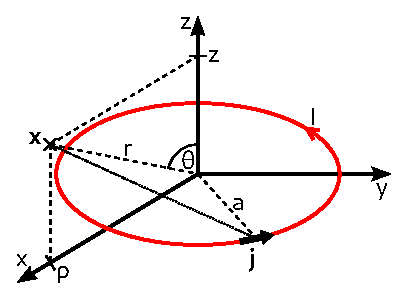
\includegraphics[width=0.5\textwidth]{img/circularWireLoop.eps}
 \caption{Geometry of a circular wire loop centered at the origin with normal vector aligned with the $z$-axis.
          The radius of the loop is denoted $a$ and a current $I$ flows in the indicated direction.
          The magnetic field and vector potential are to be evaluated at the point $\mathbf{x}$ in the ($x$, $z$)-plane.}
 \label{fig:circularWireLoop}
\end{figure}

Similar to the case of the straight wire segment,
the magnetic vector potential and the magnetic field of the circular wire loop
are assembled from various formulations for special cases of the far-field and the near-field.

\subsubsection{Magnetic Vector Potential}
The magnetic vector potential of a circular wire loop
only has a tangential component~$A_\varphi$.
In Eqn.~(5.37) of Ref.~\cite{jackson}, $A_\varphi$~is expressed as
follows for a loop of radius~$a$ and current~$I$ along it:
\begin{align}
  A_\varphi(r, \theta) &= \frac{\mu_0}{4 \pi}
                          \frac{4 I a}{\sqrt{a^2 + r^2 + 2 a r \sin(\theta)}}
                          \left[
                            \frac{(2 - k^2)\mathcal{K}(k) - 2 \mathcal{E}(k)}{k^2}
                          \right] \label{eqn:cwl_A_phi_Jackson}
\end{align}
with
\begin{equation}
  k^2 = \frac{4 a r \sin(\theta)}{a^2 + r^2 + 2 a r \sin(\theta)} \, .
\end{equation}
Here, $\mathcal{K}(k)$ and $\mathcal{E}(k)$ are the complete elliptic integrals of the first and second kind, respectively.
Spherical coordinates~$(r, \theta)$ are used to specify the evaluation location.
The corresponding cylindrical coordinates~$(\rho, z)$ are given by
$\rho = r \sin(\theta)$ and $z = \sqrt{r^2 - \rho^2}$.
Normalized coordinates are used with
\begin{align}
  \rho' = \rho / a \label{eqn:rhoP} \\
    z'  =   z  / a \label{eqn:zP} \, .
\end{align}
An expression for the linear combination of $\mathcal{K}(k)$ and $\mathcal{E}(k)$ from Ref.~\cite{bulirsch_3}
is used to reformulate the expression provided by Jackson:
\begin{equation}
  \lambda \mathcal{K}(k) + \mu \mathcal{E}(k) = \,\mathrm{cel}(k_c, 1, \lambda + \mu, \lambda + \mu k_c^2)
\end{equation}
where
\begin{equation}
  k_\mathrm{c}^2 = 1 - k^2 \, .
\end{equation}
The argument of the elliptic integrals is considered first:
\begin{align}
  k^2 &= \frac{4 a r \sin(\theta)}{a^2 + r^2 + 2 a r \sin(\theta)}
       = \frac{4 a \rho}{a^2 + r^2 + 2 a \rho}
       = \frac{4 \bcancel{a} \rho}{a^{\bcancel{2}} \left(1 + \frac{r^2}{a^2} + 2 \frac{\rho}{a} \right)} \nonumber \\
  ~   &= \frac{4 \rho'}{1 + \frac{r^2}{a^2} + 2 \rho'}
       = 4 \rho' \left( 1 + \frac{\rho^2 + z^2}{a^2} + 2 \rho' \right)^{-1} \nonumber \\
  ~   &= 4 \rho' \left( 1 + \rho'^{2} + z'^{2} + 2 \rho' \right)^{-1}
       = \frac{4 \rho'}{z'^2 + (1 + \rho')^2} \, . \label{eqn:kSq}
\end{align}
This implies:
\begin{equation}
  k_c^2 = \frac{z'^2 + (1 - \rho')^2}{z'^2 + (1 + \rho')^2} \, . \label{eqn:kCSq_general}
\end{equation}
The coefficients of the elliptic integrals are identified as follows:
\begin{align}
  \lambda &= \frac{2 - k^2}{k^2} = \frac{2}{k^2} - 1 \\
  \mu     &= -\frac{2}{k^2}
\end{align}
and their combinations are as follows:
\begin{align}
  \lambda + \mu       &= \frac{2}{k^2} - 1 - \frac{2}{k^2}     = -1 \\
  \lambda + \mu k_c^2 &= \frac{2}{k^2} - 1 - \frac{2}{k^2} (1 - k^2) \nonumber \\
          ~           &= \frac{2}{k^2} - 1 - \frac{2}{k^2} + 2 =  1 \, .
\end{align}
Putting above results together, we arrive at the following expression for $A_\varphi$:
\begin{equation}
 A_\varphi(\rho', z') = \frac{\mu_0 I}{\pi}
                        \frac{1}{\sqrt{z'^2 + (1 + \rho')^2}} \,\mathrm{cel}(k_c, 1, -1, 1) \, . \label{eqn:cwl_A_phi_cel}
\end{equation}
It is favorable for numerical evaluation of $A_\varphi$ to use the form given in \eqn{cwl_A_phi_cel}
where the linear combination of the complete elliptic integrals is embedded in the parameters of $\mathrm{cel}(k_c, p, a, b)$
and less precautions need to be taken to deal with cancellations in \eqn{cwl_A_phi_Jackson}.
A physics-oriented prefactor is split off to be able to focus on geometry in the following:
\begin{equation}
  A_\varphi(\rho', z') = \frac{\mu_0 I}{\pi} \tilde{A}_\varphi(\rho',z') \label{eqn:norm_A_phi}
\end{equation}
with
\begin{equation}
  \tilde{A}_\varphi(\rho',z')
  = \frac{1}{\sqrt{z'^2 + (1 + \rho')^2}} \,\mathrm{cel}(k_c, 1, -1, 1) \, .
\end{equation}
One of several formulations is chosen depending on the evaluation location~$(\rho', z')$:
\begin{equation}
  \tilde{A}_\varphi (\rho', z') =
  \begin{cases}
    0                                          &:\, \rho' = 0 , \textrm{ any } z' \\
    \tilde{A}_{\varphi,\mathrm{f}} (\rho', z') &:\, \rho' < 1/2 \textrm{ or } \rho' > 2 \textrm{ or } |z'| \geq 1 \\
    \tilde{A}_{\varphi,\mathrm{n}} (\rho', z') &:\, 1/2 \leq \rho' \leq 2 \textrm{ but } \rho' \neq 1, |z'| < 1 \\
    \tilde{A}_{\varphi,\mathrm{v}} (\rho', z') &:\, \textrm{else} \, .
  \end{cases} \label{eqn:A_phi_final}
\end{equation}
The following formula is implemented for evaluation locations away from the wire loop:
\begin{equation}
  \tilde{A}_{\varphi,\mathrm{f}} (\rho',z')
  = \frac{k^2}{\sqrt{z'^2 + (1 + \rho')^2}} \,\mathcal{C}(k_c) \label{eqn:cwl_A_phi_f}
\end{equation}
with $k^2$~from~\eqn{kSq} and
\begin{equation}
  \mathcal{C}(k_c)
  = \,\mathrm{cel} \left( \frac{2 \sqrt{k_c}}{1 + k_c}, 1, 0, \frac{2}{(1 + k_c)^3} \right) \, . \label{eqn:elliptic_c}
\end{equation}
Close to the wire loop, the following formulation is used:
\begin{equation}
  \tilde{A}_{\varphi,\mathrm{n}} (\rho',z')
  = \frac{1}{|\rho' - 1| \sqrt{\left( \frac{z'}{\rho'-1} \right)^2 + \left(1 + \frac{2}{\rho'-1} \right)^2 }}
    \,\mathrm{cel}(\sqrt{k_c^2}, 1, -1, 1) \label{eqn:cwl_A_phi_n}
\end{equation}
with $k_c^2$ computed as follows:
\begin{equation}
  k_c^2 = \frac{\left( \frac{z'}{\rho'-1} \right)^2 + 1}{\left( \frac{z'}{\rho'-1} \right)^2 + \left(1 + \frac{2}{\rho'-1} \right)^2} \, .
\end{equation}
At~$\rho' = 1$, some further simplification can be carried out.
This leads to the following formulation for~$\rho' = 1$ and~$|z'| < 1$:
\begin{equation}
  \tilde{A}_{\varphi,\mathrm{v}} (\rho'=1, z') = \frac{1}{|z'|} \,\mathrm{cel}\left(\frac{1}{k_c}, 1, 1, -1\right) \label{eqn:cwl_A_phi_v}
\end{equation}
with $k_c$ computed as follows:
\begin{equation}
  k_c = \frac{|z'|}{\sqrt{4 + {z'}^2}} \, .
\end{equation}

\subsubsection{Magnetic Field}
The magnetic field produced by a circular wire loop is made up of two components:
$B_\rho$ denotes the radial component and $B_z$ denotes the vertical component.
The radial component~$B_\rho$ is given by:
\begin{equation}
  B_\rho(\rho', z')
  = \frac{\mu_0 I}{\pi a} \frac{z'}{\left[ z'^2 + (1 + \rho')^2 \right]^{\frac{3}{2}}} \,\mathrm{cel}(k_c, k_c^2, -1, 1)
\end{equation}
Also here, a normalization factor is split off:
\begin{equation}
  B_\rho(\rho, z) = \frac{\mu_0 I}{\pi a} \tilde{B}_\rho(\rho', z')
\end{equation}
with
\begin{align}
  \tilde{B}_\rho(\rho', z')
  =&\, \frac{z'}{\left[ z'^2 + (1 + \rho')^2 \right]^{\frac{3}{2}}} \,\mathrm{cel}(k_c, k_c^2, -1, 1) \, .
\end{align}
One of several formulations is chosen depending on the evaluation location~$(\rho', z')$:
\begin{equation}
  \tilde{B}_\rho(\rho', z')
  = \begin{cases}
      0                                 &:\, \rho' = 0, \textrm{ any } z' \\
                    ~                   &\, ~\textrm{ or any } \rho', z' = 0 \\
      \tilde{B}_{\rho,\mathrm{f}} (\rho', z') &:\, \rho' < 1/2 \textrm{ or } \rho' > 2 \textrm{ or } |z'| \geq 1 \\
      \tilde{B}_{\rho,\mathrm{n}} (\rho', z') &:\, 1/2 \leq \rho' \leq 2 \textrm{ but } \rho' \neq 1, |z'| < 1 \\
      \tilde{B}_{\rho,\mathrm{v}} (z')        &:\, \textrm{else} \, .
    \end{cases}
\end{equation}
The following formulation is implemented for evaluation locations away from to the wire loop:
\begin{equation}
  \tilde{B}_{\rho,\mathrm{f}} (\rho', z')
  = \frac{4 \rho' z' \left[ \,\mathcal{D}(k_c) - \,\mathcal{C}(k_c) \right]}
         {\left[{z'}^2 + (1 + \rho')^2 \right]^{3/2} \left[{z'}^2 + (1 - \rho')^2 \right] } \label{eqn:cwl_B_rho_f}
\end{equation}
with
\begin{equation}
  \mathcal{D}(k_c)
  = \frac{\mathcal{K}(k_c) - \,\mathcal{E}(k_c)}{k^2}
  = \,\mathrm{cel}(k_c, 1, 0, 1) \, . \label{eqn:elliptic_d}
\end{equation}
For points close to the wire loop, but with~$\rho' \neq 1$, the following formulation is used:
\begin{align}
  \tilde{B}_{\rho,\mathrm{n}}& (\rho', z')
  = \frac{4 \rho' \left|\frac{z'}{\rho'-1}\right| \left[ \,\mathcal{D}(k_c) - \,\mathcal{C}(k_c) \right]}
         {(\rho' - 1)^4} \nonumber \\
  ~& \left\{
      \left[ \left( \frac{z'}{\rho'-1} \right)^2 + \left(1 + \frac{2}{\rho'-1} \right)^2 \right]^{3/2}
      \left[ \left( \frac{z'}{\rho'-1} \right)^2 + 1 \right]
    \right\}^{-1} \label{eqn:cwl_B_rho_n} \, .
\end{align}
Finally, for $\rho'=1$ and~$|z'| < 1$, the following formulation is used:
\begin{equation}
  \tilde{B}_{\rho,\mathrm{v}} (z')
  = \frac{1}{2 \sqrt{1 + 4/{z'}^2}}
    \left[  \frac{\mathcal{E}(k_c)}{1 + 4/{z'}^2} \left( 1 + \frac{1}{{z'}^2} \left( 6 + \frac{8}{{z'}^2} \right) \right)
            - \mathcal{K}(k_c) \right]
\end{equation}
with
\begin{equation}
  k_c^2 = \frac{1}{1 + 4/{z'}^2} \, .
\end{equation}
The vertical component~$B_z$ of the magnetic field of a circular wire loop is given by:
\begin{align}
 B_z(\rho', z')
 =&\, \frac{\mu_0 I}{2 \pi a}
   \frac{1}{\rho' \sqrt{z'^2 + (1 + \rho')^2}} \nonumber \\
 ~& \left[
       \textrm{cel}(k_c, 1, -1, 1)
     + \frac{1 + k_c^2 - \left( 1 - k_c^2 \right) \rho'}{2} \textrm{cel}(k_c, k_c^2, -1, 1)
   \right]
\end{align}
One of several formulations is selected depending on the evaluation location~$(\rho', z')$:
\begin{equation}
  \tilde{B}_z(\rho', z')
  = \begin{cases}
      \tilde{B}_{z,1} (\rho', z') &:\, \rho' < 1/2 \textrm{ or } (\rho' < 2 \textrm{ and } z' \geq 1) \\
      \tilde{B}_{z,2} (\rho', z') &:\, \rho' \geq 2 \\
      \tilde{B}_{z,4} (\rho', z') &:\, \rho' = 1 \\
      \tilde{B}_{z,5} (\rho', z') &:\, z' \neq 0 \\
      \tilde{B}_{z,6} (\rho', z') &:\, \textrm{else}
    \end{cases} \, .
\end{equation}






{\color{red}
TODO: There is a factor of 2 too much in the denominator of $B_z$!
}

Finally, a normalization factor is split off here as well:
\begin{equation}
  B_z(\rho, z) = \frac{\mu_0 I}{2 \pi a} \tilde{B}_z(\rho', z')
\end{equation}
with
\begin{align}
  \tilde{B}_z(\rho', z')
  =&\, \frac{1}{\rho' \sqrt{z'^2 + (1 + \rho')^2}} \nonumber \\
 ~& \left[
       \textrm{cel}(k_c, 1, -1, 1)
     + \frac{1 + k_c^2 - \left( 1 - k_c^2 \right) \rho'}{2} \textrm{cel}(k_c, k_c^2, -1, 1)
   \right] \, .
\end{align}
The evaluation of this formula is split up as well into separate special cases.
For points not too close to the wire loop,
the following formulation is used:
\begin{align}
  \tilde{B}_{z,1} (\rho', z')
  =&\, \frac{1}{\sqrt{{z'}^2 + (1+\rho')^2} \left[{z'}^2 + (1 - \rho')^2 \right] } \nonumber \\
  ~&\,  \left[ \mathcal{E}(k_c) + \rho' \left( \mathcal{E}(k_c) - 2 \mathcal{K}(k_c) + 2 \mathcal{D}(k_c) \right) \right] \, .
\end{align}
A second method is needed for points with $\rho' > 2$:
\begin{equation}
  \tilde{B}_{z,2} (\rho', z')
  = \frac{1}{\sqrt{r_0} {\rho'}^3}
    \left[ \mathcal{E}(k_c) + \frac{4}{t} \left( \mathcal{C}(k_c) - \,\mathcal{D}(k_c) \right) \right]
\end{equation}
with
\begin{align}
  r_0
  = &\,             1 + \frac{1}{\rho'} \Biggl[
                  - 2 + \frac{1}{\rho'} \Biggl(
         3 {z'}^2 - 1 + \frac{1}{\rho'} \Biggl\{
       - 4 {z'}^2 + 4 \nonumber \\
  ~& + \frac{1}{\rho'} \Biggl[ 3 \left( {z'}^2 + 1 \right)^2 - 4 \left( {z'}^2 + 1 \right) \nonumber \\
  ~& + \frac{1}{\rho'} \Biggl(-2 \left( {z'}^2 + 1 \right)^2 + \frac{1}{\rho'} \left( {z'}^2 + 1 \right)^3
       \Biggr)
       \Biggr]
       \Biggr\}
       \Biggr)
       \Biggr]
\end{align}
and
\begin{equation}
  t = 1 + \frac{1}{\rho'} \left( 2 + \frac{1}{\rho'} \left[ {z'}^2 + 1 \right] \right) \, .
\end{equation}
The expression for $\tilde{B}_z$ becomes significantly simpler at $\rho'=1$,
which is considered next:
\begin{equation}
  \tilde{B}_{z,4} (\rho'=1, z')
  = \frac{1}{\left[ {z'}^2 + 4 \right]^{3/2}} \,\mathrm{cel}(\sqrt{k_c^2}, k_c^2, 2, 0)
\end{equation}
with
\begin{equation}
  k_c^2 = \frac{{z'}^2}{{z'}^2 + 4} \, .
\end{equation}
In the vicinity of the wire loop, but explicitly obeying $z' \neq 0$,
the following method should be used to compute $\tilde{B}_z$:
\begin{equation}
  \tilde{B}_{z,5} (\rho', z')
  = \frac{\left| \frac{z'}{\rho' - 1} \right| \,\mathrm{cel}\left( \sqrt{k_c^2}, k_c^2, \frac{1 + \rho'}{z'}, \frac{1 - \rho'}{z'} \right) }
         {\left(\rho' - 1 \right)^2 \left[ \left( \frac{z'}{\rho'-1} \right)^2 + \left(1 + \frac{2}{\rho'-1} \right)^2 \right]^{3/2} } \, .
\end{equation}
Finally, only one more expression is needed to accurately compute $\tilde{B}_z$ at $z'=0$ close to the loop.
Here it is:
\begin{equation}
  \tilde{B}_{z,6} (\rho', z'=0)
  = \frac{1}{|1 + \rho'|^3}
    \,\mathrm{cel}(k_c, k_c^2, 1+\rho', 1-\rho')
\end{equation}
with
\begin{equation}
  k_c = \frac{1-\rho'}{1+\rho'} \, .
\end{equation}
%
% total assembly of B_z for circular wire loop
%






\subsection{Transformation to Cartesian Coordinates}
Evaluation of the magnetic vector potential~$A$ and magnetic field~$B$
produced by the current carriers considered in this work
happens in cylindrical coordinates~$\rho$ and~$z$.
It is often more convenient to be able to work in Cartesian coordinates.
The methods given in this section show how to transform the evaluation location
into cylindrical coordinates in the frame of reference of the current carrier
and subsequently transform back the magnetostatic quantities into the global Cartesian coordinate system.

\subsubsection{Straight Wire Segment}
Figure~\ref{fig:StraightWireSegment_MappingToCartesian} illustrates the setup of a straight wire segment.
\begin{figure}[htbp]
 \centering
 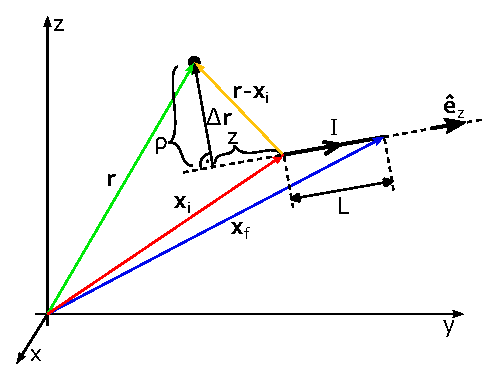
\includegraphics{img/StraightWireSegment_MappingToCartesian.eps}
 \caption{Mapping the components to Cartesian coordinates for an exemplary straight wire segment.
          The wire segment is positioned from~$\mathbf{x}_i$ to~$\mathbf{x}_f$.
          Its parallel unit vector is denoted $\hat{\mathbf{e}}_z$.
          The length of the wire segment is denoted by~$L$.
          The evaluation location is denoted by~$\mathbf{r}$.}
 \label{fig:StraightWireSegment_MappingToCartesian}
\end{figure}

The length of the wire segment is denoted by~$L$:
\begin{equation}
  L = |\mathbf{x}_f - \mathbf{x}_i| \, .
\end{equation}
The unit vector along the segment~$\hat{\mathbf{e}}_z$ is then computed as:
\begin{equation}
  \hat{\mathbf{e}}_z = \frac{\mathbf{x}_f - \mathbf{x}_i}{L} \, .
\end{equation}
The vertical coordinate~$z$ in the coordinate system of the wire segment is:
\begin{equation}
  z = (\mathbf{r} - \mathbf{x}_i) \cdot \hat{\mathbf{e}}_z
\end{equation}
and the normalized $z$-coordinate is:
\begin{equation}
  z' = \frac{z}{L} = \frac{1}{L} (\mathbf{r} - \mathbf{x}_i) \cdot \hat{\mathbf{e}}_z \, .
\end{equation}
For the radial coordinate, first the vector~$\Delta \mathbf{r}$ is formed:
\begin{equation}
  \Delta \mathbf{r} = (\mathbf{r} - \mathbf{x}_i) - z \, \hat{\mathbf{e}}_z
\end{equation}
and the radial coordinate $\rho$ is then obtained by taking $\rho = |\Delta \mathbf{r}|$.
A unit vector in radial direction is formed as follows:
\begin{equation}
  \hat{\mathbf{e}}_\rho = \frac{\Delta \mathbf{r}}{\rho} \, .
\end{equation}
The normalized radial coordinate~$\rho'$ is then obtained as:
\begin{equation}
  \rho' = \frac{\rho}{a} = \frac{1}{a} |(\mathbf{r} - \mathbf{x}_i) - z \, \hat{\mathbf{e}}_z| \, .
\end{equation}
The magnetic field of the straight wire segment consists of the tangential component~$B_\varphi$:
\begin{equation}
  \mathbf{B}(\mathbf{r}) = B_\varphi \hat{\mathbf{e}}_\varphi
\end{equation}
with $\hat{\mathbf{e}}_\varphi = \hat{\mathbf{e}}_z \times \hat{\mathbf{e}}_\rho$.
The magnetic vector potential only has a component in parallel direction in the coordinate system of the wire segment.
The vector potential of the circular wire loop in thus in Cartesian coordinates:
\begin{equation}
  \mathbf{A}(\mathbf{r}) = A_z \hat{\mathbf{e}}_z \, .
\end{equation}

\subsubsection{Circular Wire Loop}
Figure~\ref{fig:CircularWireLoop_MappingToCartesian} illustrates the setup of a circular wire loop.
\begin{figure}[htbp]
 \centering
 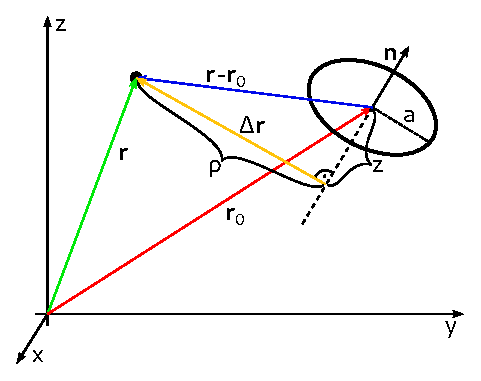
\includegraphics{img/CircularWireLoop_MappingToCartesian.eps}
 \caption{Mapping the components to Cartesian coordinates for an exemplary circular wire loop.
          The loop is centered around its origin~$\mathbf{r}_0$.
          Its normal vector is denoted $\mathbf{n}$ and defines the orientation of the loop.
          The radius of the loop is denoted by~$a$.
          The evaluation location is denoted by~$\mathbf{r}$.}
 \label{fig:CircularWireLoop_MappingToCartesian}
\end{figure}

The $z$-axis of the wire loop's coordinate system is defined by the normal vector~$\mathbf{n}$:
\begin{equation}
  \hat{\mathbf{e}}_z = \frac{\mathbf{n}}{|\mathbf{n}|} \, .
\end{equation}
The $z$ component of the evaluation location is thus obtained as follows:
\begin{equation}
  z = (\mathbf{r} - \mathbf{r}_0) \cdot \hat{\mathbf{e}}_z \, .
\end{equation}
The normalized $z$-coordinate $z'$ is then obtained as:
\begin{equation}
  z' = \frac{z}{a} = \frac{1}{a} (\mathbf{r} - \mathbf{r}_0) \cdot \hat{\mathbf{e}}_z \, .
\end{equation}
For the radial coordinate, first the vector~$\Delta \mathbf{r}$ is formed:
\begin{equation}
  \Delta \mathbf{r} = (\mathbf{r} - \mathbf{r}_0) - z \, \hat{\mathbf{e}}_z
\end{equation}
and the radial coordinate $\rho$ is then obtained by taking $\rho = |\Delta \mathbf{r}|$.
A unit vector in radial direction is formed as follows:
\begin{equation}
  \hat{\mathbf{e}}_\rho = \frac{\Delta \mathbf{r}}{\rho} \, .
\end{equation}
The normalized radial coordinate~$\rho'$ is then obtained as:
\begin{equation}
  \rho' = \frac{\rho}{a} = \frac{1}{a} |(\mathbf{r} - \mathbf{r}_0) - z \, \hat{\mathbf{e}}_z| \, .
\end{equation}
The magnetic field of the circular wire loop consists of two cylindrical components, namely $B_\rho$ and $B_z$.
The Cartesian magnetic field components are then computed as follows:
\begin{equation}
  \mathbf{B}(\mathbf{r}) = B_\rho \hat{\mathbf{e}}_\rho + B_z \hat{\mathbf{e}}_z \, .
\end{equation}
The magnetic vector potential only has a component in angular direction in the coordinate system of the wire loop.
The corresponding unit vector~$\hat{\mathbf{e}}_\varphi$ is then given by
$\hat{\mathbf{e}}_\varphi = \hat{\mathbf{e}}_z \times \hat{\mathbf{e}}_\rho$.
The vector potential of the circular wire loop in thus in Cartesian coordinates:
\begin{equation}
  \mathbf{A}(\mathbf{r}) = A_\varphi \hat{\mathbf{e}}_\varphi \, .
\end{equation}

\subsection{Superposition in multi-filament assemblies}

% PolygonFilament

An infinitely thin polygon filament $P$ is described by a list of $N$ points $\mathbf{x}_i$ with $i=1, ..., N$ in three-dimensional (3D) space and a current $I$.
The $(N-1)$ straight connecting lines between each two consecutive points $\mathbf{x}_i$ and $\mathbf{x}_{i+1}$ are assumed to represent the geometry of a wire which carries the current.
If the first and the last point of the polygon filament coincide, the wire forms a closed loop and $\nabla \cdot \mathbf{j} = 0$ is ensured by construction.

The magnetic vector potential $\mathbf{A}(I, \mathbf{x}_i, \mathbf{x}_{i+1}, \mathbf{x})$ and the magnetic field $\mathbf{B}(I, \mathbf{x}_i, \mathbf{x}_{i+1}, \mathbf{x})$
of the wire segments at a location $\mathbf{x}$ can be computed analytically.
The resulting contributions from each segment are superposed in order to compute the resulting magnetic field from the full length of the wire:
\begin{align}
 \mathbf{A}(\mathbf{x}) & = \sum_{i=1}^{N-1} \mathbf{A}(I, \mathbf{x}_i, \mathbf{x}_{i+1}, \mathbf{x}) \quad \mathrm{and} \\
 \mathbf{B}(\mathbf{x}) & = \sum_{i=1}^{N-1} \mathbf{B}(I, \mathbf{x}_i, \mathbf{x}_{i+1}, \mathbf{x}) \quad .
\end{align}
Computationally robust and efficient expressions for
$\mathbf{A}(I, \mathbf{x}_i, \mathbf{x}_{i+1}, \mathbf{x})$ and
$\mathbf{B}(I, \mathbf{x}_i, \mathbf{x}_{i+1}, \mathbf{x})$
are given in Ref.~\cite{hanson_hirshman_2002}.
The detailed derivation of these expressions is given below.

% Kahan-Babuska summation



\subsection{Verification Method}
The asymptotic behavior of an implementation of above formulas for the magnetic vector potential
and magnetic field needs to be tested before using that implementation in daily routine work.

A set of critical test points used to check this is shown in Fig.~\ref{fig:circularLoop_criticalPoints}
for the case of the circular wire loop.
\begin{figure}[htbp]
 \centering
 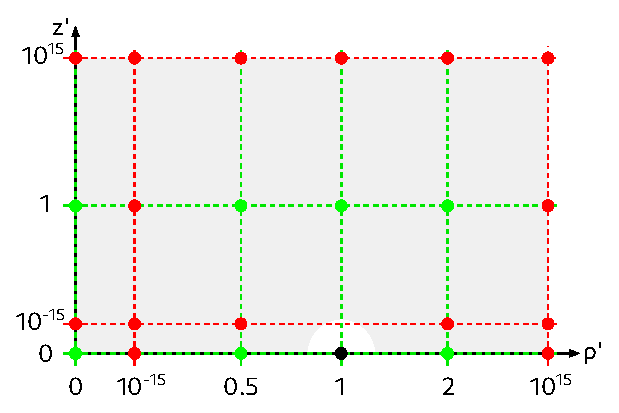
\includegraphics{img/circularLoop_criticalPoints.eps}
 \caption{Test points in the $R$-$Z$-plane for a circular wire loop (black dot).
          The axes are labeled in normalized cylindrical coordinates ($\rho' = \rho / a$, $z' = z / a$; $a$ is the radius of the wire loop).
          Green dashed lines indicate values of $\rho'$ and $z'$ which are well handled by a naive implementation.
          Green dots denote points at which a naive implementation yields satisfactory results.
          Red dashed lines indicate values of $\rho'$ and $z'$ which induce the requirement for robust asymptotic behavior.
          Red dots denote points at which a naive implementation usually fails.
          The grey shaded area in the background indicates the region in which the reference implementation yields accurate results.
          Note that the problem is symmetric in $z$ direction, even though only the positive-$z$ quadrant is considered here.}
 \label{fig:circularLoop_criticalPoints}
\end{figure}

The reference results are computed on each test point using arbitrary-precision arithmetic
as provided by the Python package~\texttt{mpmath}~\cite{mpmath} and Mathematica~\cite{Mathematica}.
The test point coordinates are computed within the finite-precision test programs used to check the accuracy of the results.
This implies that the exact \textit{implied} values of the test point coordinates have to be transported
into the arbitrary-precision software used to compute the reference data.
The evaluation positions are specified at IEEE754~\texttt{float64} floating-point numbers.
The floating point numbers are re-constructed within the arbitrary-precision software
in order to properly transport their intended value.
In case of \texttt{float64}, this is done as follows for a floating-point number~$f$:
\begin{equation}
 f = \begin{cases}
      0                                                             & E=0 \textrm{ and } M=0 \\
      (-1)^s \, 2^{E - 1023} \, \left( 1 + \frac{M}{2^{52}} \right) & \textrm{else}
     \end{cases}
     \label{eqn:float64}
\end{equation}
where $s$ is the sign bit, $E$ is the exponent specified as an 11-bit unsigned integer
and $M$ is the mantissa specified as a 52-bit unsigned integer.
Several special cases are defined for certain values of $s$, $E$ and $M$,
but in the context of this work only the case $E=0$, $M=0$ ($s$ arbitrary),
which represents an exact zero, is relevant.
The organization of those bits in a \texttt{float64} number is shown in Fig.~\ref{fig:float64}.
\begin{figure}[htbp]
 \centering
 \includegraphics{img/IEEE754_float64.eps}
 \caption{Organization of sign bit~$s$, exponent~$E$ (11 bits, unsigned integer)
          and mantissa~$M$ (52 bits, unsigned integer) within the 64 bits
          of a IEEE754~\texttt{float64} floating-point number.
          Each box represents one bit and the colors indicate which quantity a bit belongs to
          (red: sign bit, green: exponent, blue: mantiassa).}
 \label{fig:float64}
\end{figure}
In particular, a test point coordinate value~$f$ is passed to the reference computation
by passing the three values $s$, $E$ and $M$ as integers (which are easy to represent exactly).
Within the reference computation, the value of $f$ is constructed using~\eqn{float64} implemented
in arbitrary precision and with the exact values of $s$, $E$ and $M$.


The reference data for the straight wire segment methods
is computed using 300 decimal digits of precision.
The reference data for the circular wire loop
is computed using 200 decimal digits of precision.


The evaluation position is specified exactly
via $s_\rho$, $E_\rho$ and $M_\rho$ (for $\rho'$)
and $s_z$, $E_z$ and $M_z$ (for $z'$):
\begin{align}
 \rho' \leftarrow&\, (-1)^{s_\rho} \, 2^{E_\rho - 1023} \, \left(1 + \frac{M_\rho}{2^{52}}  \right) \nonumber \\
    z' \leftarrow&\, (-1)^{s_z   } \, 2^{E_z    - 1023} \, \left(1 + \frac{M_z   }{2^{52}}  \right)
\end{align}
The following algorithm is used to compute reference values
of $\tilde{A}_z$ and $\tilde{B}_\varphi$ at~$(\rho', z')$
for the straight wire segment:
\begin{align}
  r_\mathrm{i}  \leftarrow&\, \sqrt{ {\rho'}^2 + {z'}^2 } \nonumber \\
  r_\mathrm{f}  \leftarrow&\, \sqrt{ {\rho'}^2 + \left(1 - z'\right)^2 } \label{alg:sws_ref} \\
  \epsilon \leftarrow&\, \left( r_\mathrm{i} + r_\mathrm{f} \right)^{-1} \nonumber \\
  \tilde{A}_z \leftarrow&\, \textrm{atanh} (\epsilon) \nonumber \\
  \tilde{B}_\varphi \leftarrow&\, \left(\frac{1}{r_\mathrm{i}} + \frac{1}{r_\mathrm{f}} \right) \frac{\rho'}{r_\mathrm{i} r_\mathrm{f} + {\rho'}^2 + z' (z' - 1)} \nonumber
\end{align}
The following algorithm is used to compute reference values
of $\tilde{A}_\varphi$ and $\tilde{B}_\rho$ at~$(\rho', z')$
for the circular wire loop:
\begin{align}
 k_c^2 \leftarrow&\, \frac{{z'}^2 + \left(1 - \rho'\right)^2}{{z'}^2 + \left(1 + \rho'\right)^2} \nonumber \\
 \textrm{if } \rho' =&\, 0 : \tilde{A}_\varphi = 0 ; \textrm{else:} \nonumber \\
 \tilde{A}_\varphi \leftarrow&\,
     \frac{1}{\sqrt{{z'}^2 + \left(1 + \rho'\right)^2}}
                                 \int\limits_0^{\pi/2}
                                   \frac{\sin^2(\varphi) - \cos^2(\varphi)}
                                        {\sqrt{\cos^2(\varphi) + k_c^2 \sin^2(\varphi)}} \,\mathrm{d}\varphi \label{eqn:A_phi_ref} \\
 \textrm{if } \rho' =&\, 0 \textrm{ or } z' = 0 : \tilde{B}_\rho = 0 ; \textrm{else:} \nonumber \\
 \tilde{B}_\rho \leftarrow&\,
    \frac{z'}{\left[{z'}^2 + \left(1 + \rho'\right)^2\right]^{3/2}}
                                 \int\limits_0^{\pi/2}
                                   \frac{\sin^2(\varphi) - \cos^2(\varphi)}
                                        {\left[\cos^2(\varphi) + k_c^2 \sin^2(\varphi)\right]^{3/2}} \,\mathrm{d}\varphi
\end{align}
The method used to compute $\tilde{B}_z$ works slightly differently:
\begin{align}
 k^2 \leftarrow&\,
  \begin{cases}
    4 / \left( \frac{1}{\rho'} + 2 + \rho' \right) &\, z' = 0 \\
    \frac{4 \rho'}{{z'}^2 + \left(1 + \rho'\right)^2} &\, \textrm{else}
  \end{cases} \nonumber \\
 \tilde{B}_z \leftarrow&\,
   \frac{1}{\left[ {z'}^2 + \left(1 + \rho'\right)^2 \right]^{3/2} }
                                 \int\limits_0^{\pi/2}
                                   \frac{(1-\rho') \sin^2(\varphi) + (1+\rho') \cos^2(\varphi)}
                                        {\left[1 - k^2 \sin^2(\varphi) \right]^{3/2}} \,\mathrm{d}\varphi
\end{align}
The integrals are carried out numerically within the arbitrary-precision software.
In case of~\texttt{mpmath}, double-exponential quadrature~\cite{double_exp_quad} is used~\cite{mpmath_quad}.




The error metric employed in this work is given as follows:
\begin{equation}
 \delta(a, b)
 = \begin{cases}
    \log_{10} \left(\min\left(1, \left| \frac{a - b}{b} \right|\right) \right) & b \neq 0, a \neq b \\
    0                                                                          & b=0, a \neq 0 \\
    -16                                                                        & \textrm{else}
   \end{cases}
\end{equation}


